%\cia\vspace{-2cm}
\subsection{Time of flight smearing}
The GSIM simulation of the TOF detector 
presents finer resolution
than for real data.
This is shown in \F{fig:sc_comp1} where the TOF proton mass $M^2$, 
calculated as in Section \ref{sec:proton_id},
is plotted for real data and MonteCarlo events.
Since the proton identification is based on $M$, it is important that the simulation reproduces
this quantity precisely. 

It was found that the mean position of $M^2$ differs between data and simulation due to an imperfect
calibration\footnote{The TOF is calibrated using electrons and pions as reference.
                    As a consequence the protons timing is shifted. }.
This is not important because the cuts include such a shift.

\begin{figure}[h]
 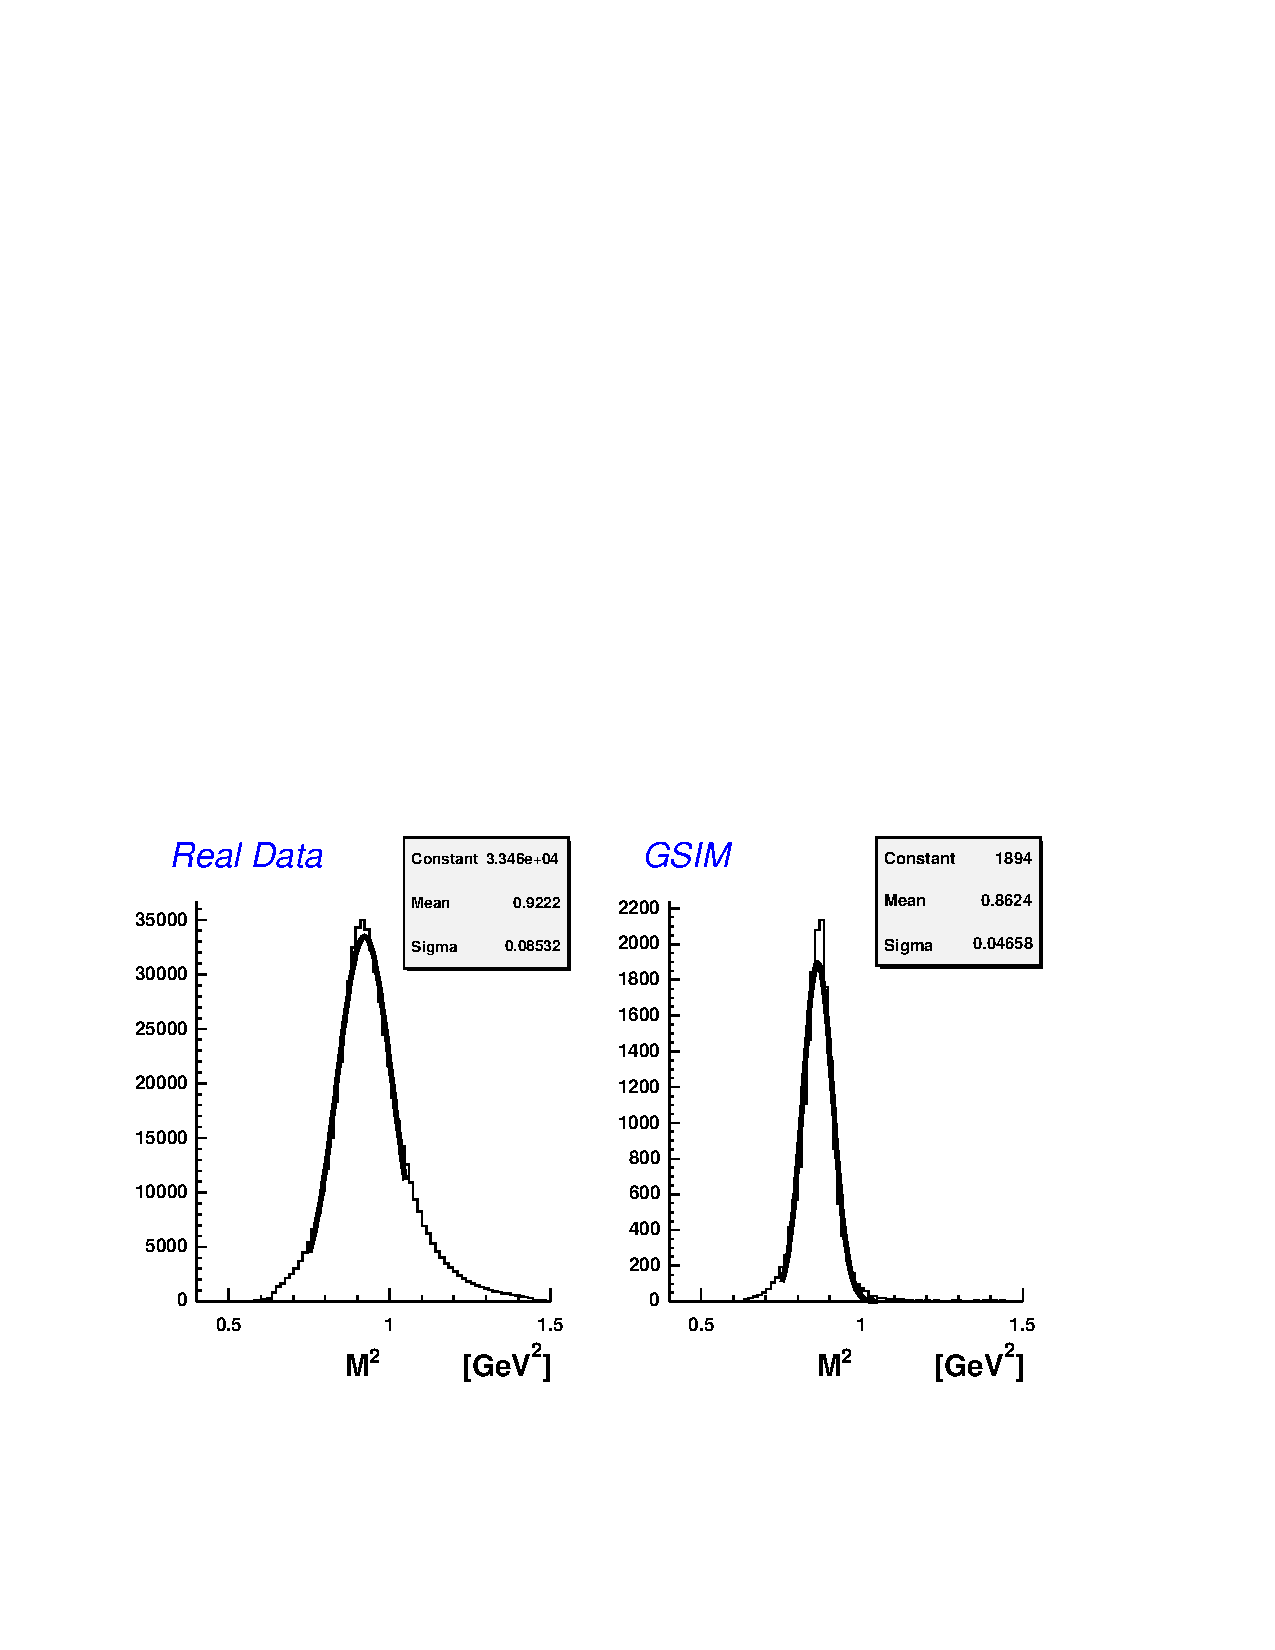
\includegraphics[width = 15.4cm, bb=0 100 500 430]{acceptance/img/comp1_sc}
 \caption[Square of TOF mass $M^2$]
         { Square of TOF mass $M^2$. Left: real data 
		    $\pi^0$ events. Right: MonteCarlo MAID 2000 simulation. The mean position is different
		    due to imperfect calibration of the TOF bars
                    . The MonteCarlo data show a finer resolution:
		    $\sigma_{REAL} = 0.085$ GeV$^2$ while $\sigma_{GSIM} = 0.047$ GeV$^2$.}
 \label{fig:sc_comp1}
\end{figure}
However the simulation should show the same resolution if one wants to make sure that the background
is handled in the same way as the real data.
In order to smear the GSIM TOF a realistic $\sigma$ from a calibration study \cite{bib:tof} 
shown in \F{fig:fit_laser} was used.
The function shown in the plot makes sure that the response of the MonteCarlo TOF resembles
the real data case.
\begin{figure}[h]
 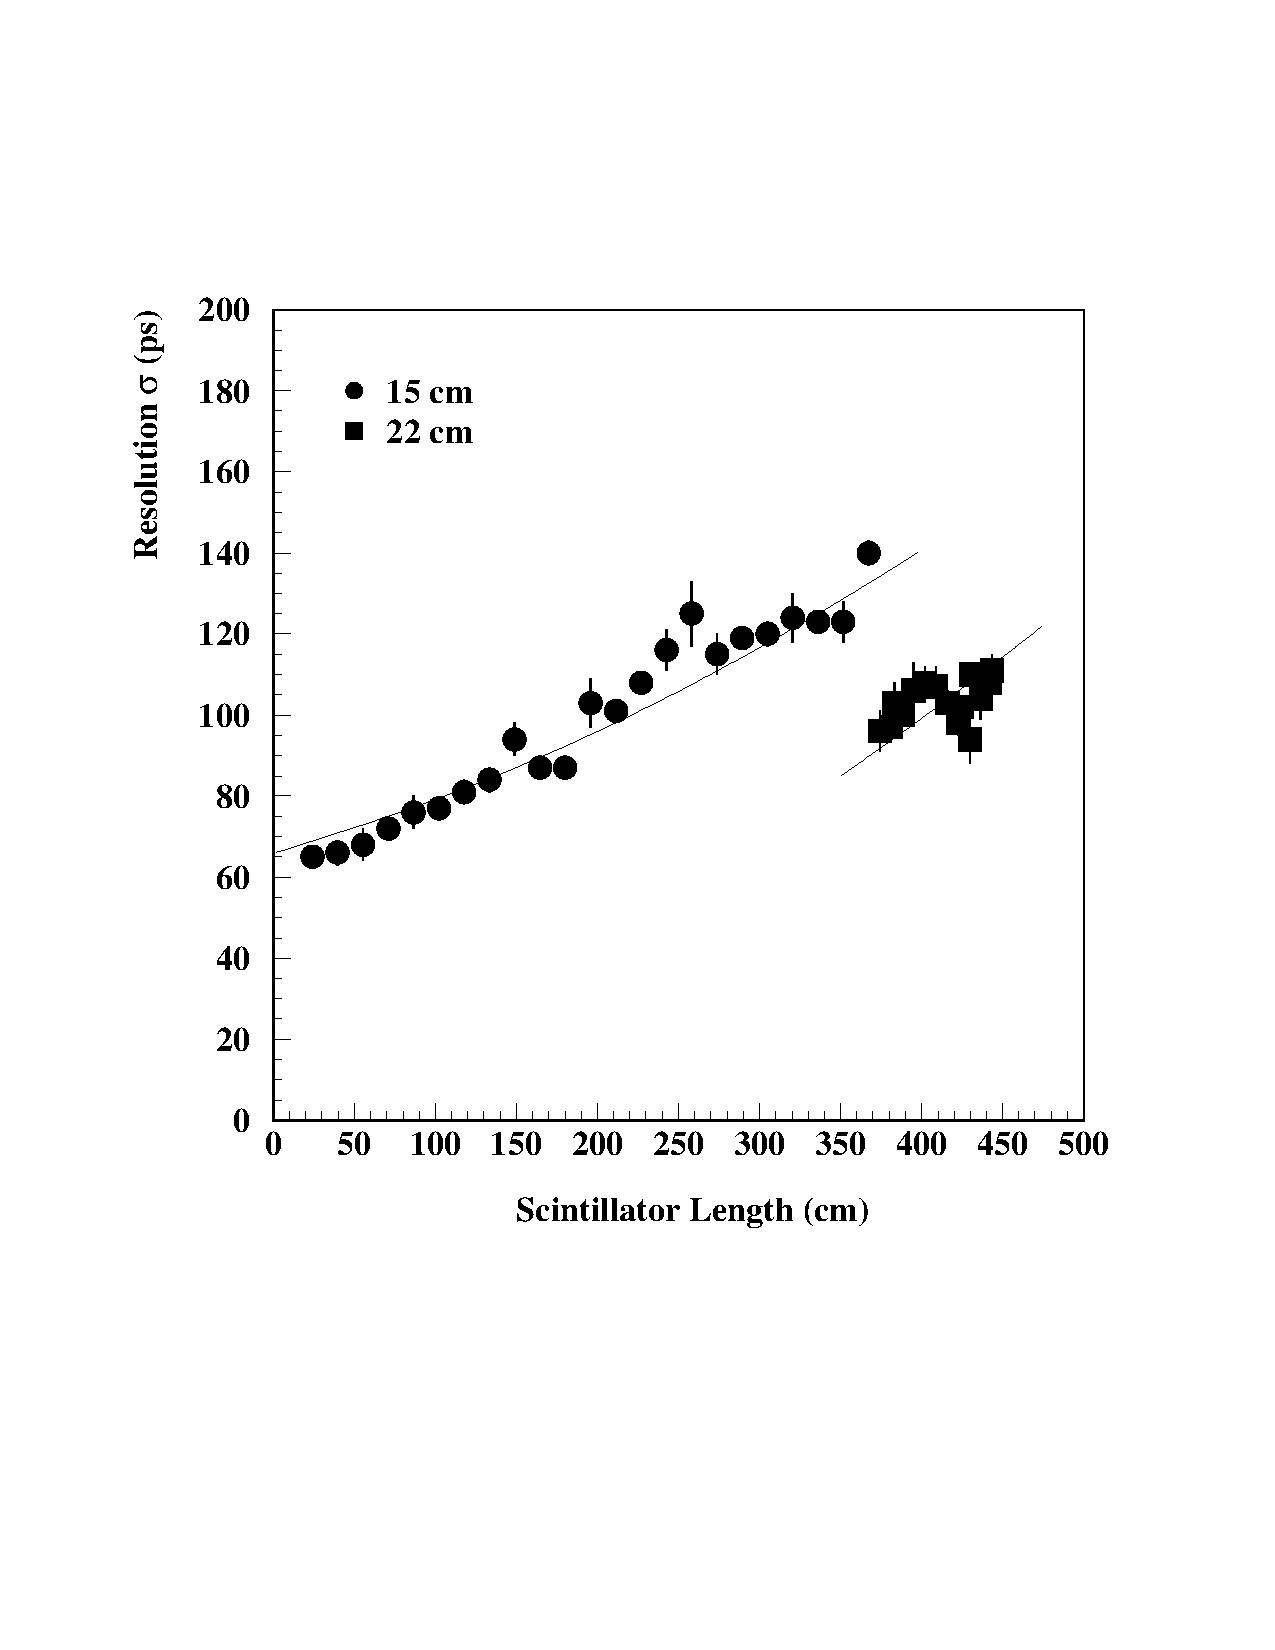
\includegraphics[width = 13cm, bb=-110 180 610 700]{acceptance/img/fit_laser_sigma}
 \caption[The timing resolution as determined from cosmic ray tests]
         { The timing resolution as determined from cosmic ray tests (see \cite{bib:tof}
	            for details). The curve represent the resolution (for two different paddle sizes)
		    used to smear the MonteCarlo TOF response. }
 \label{fig:fit_laser}
\end{figure}

In order to perfectly match the real data and MonteCarlo TOF resolution 
a few simulations of 20,000 events each were performed. In each simulation 
the function in \F{fig:fit_laser}
was multiplied by a trial number $f$ (from $0.5$ to $1.4$) and used to smear the TOF signal.
In each case the resulting TOF mass  was fitted
with a gaussian and the obtained $\sigma$ are plotted versus the multiplicative number $f$.
This is shown  in \F{fig:tof_fit}
where the real data $\sigma$ are also plotted. One can clearly see that $\sigma$ is linear
with $f$. 

The value $f=1.35$ matches the real data resolution and therefore is the value used throughout all
the GSIM simulation.

\begin{figure}[t]
 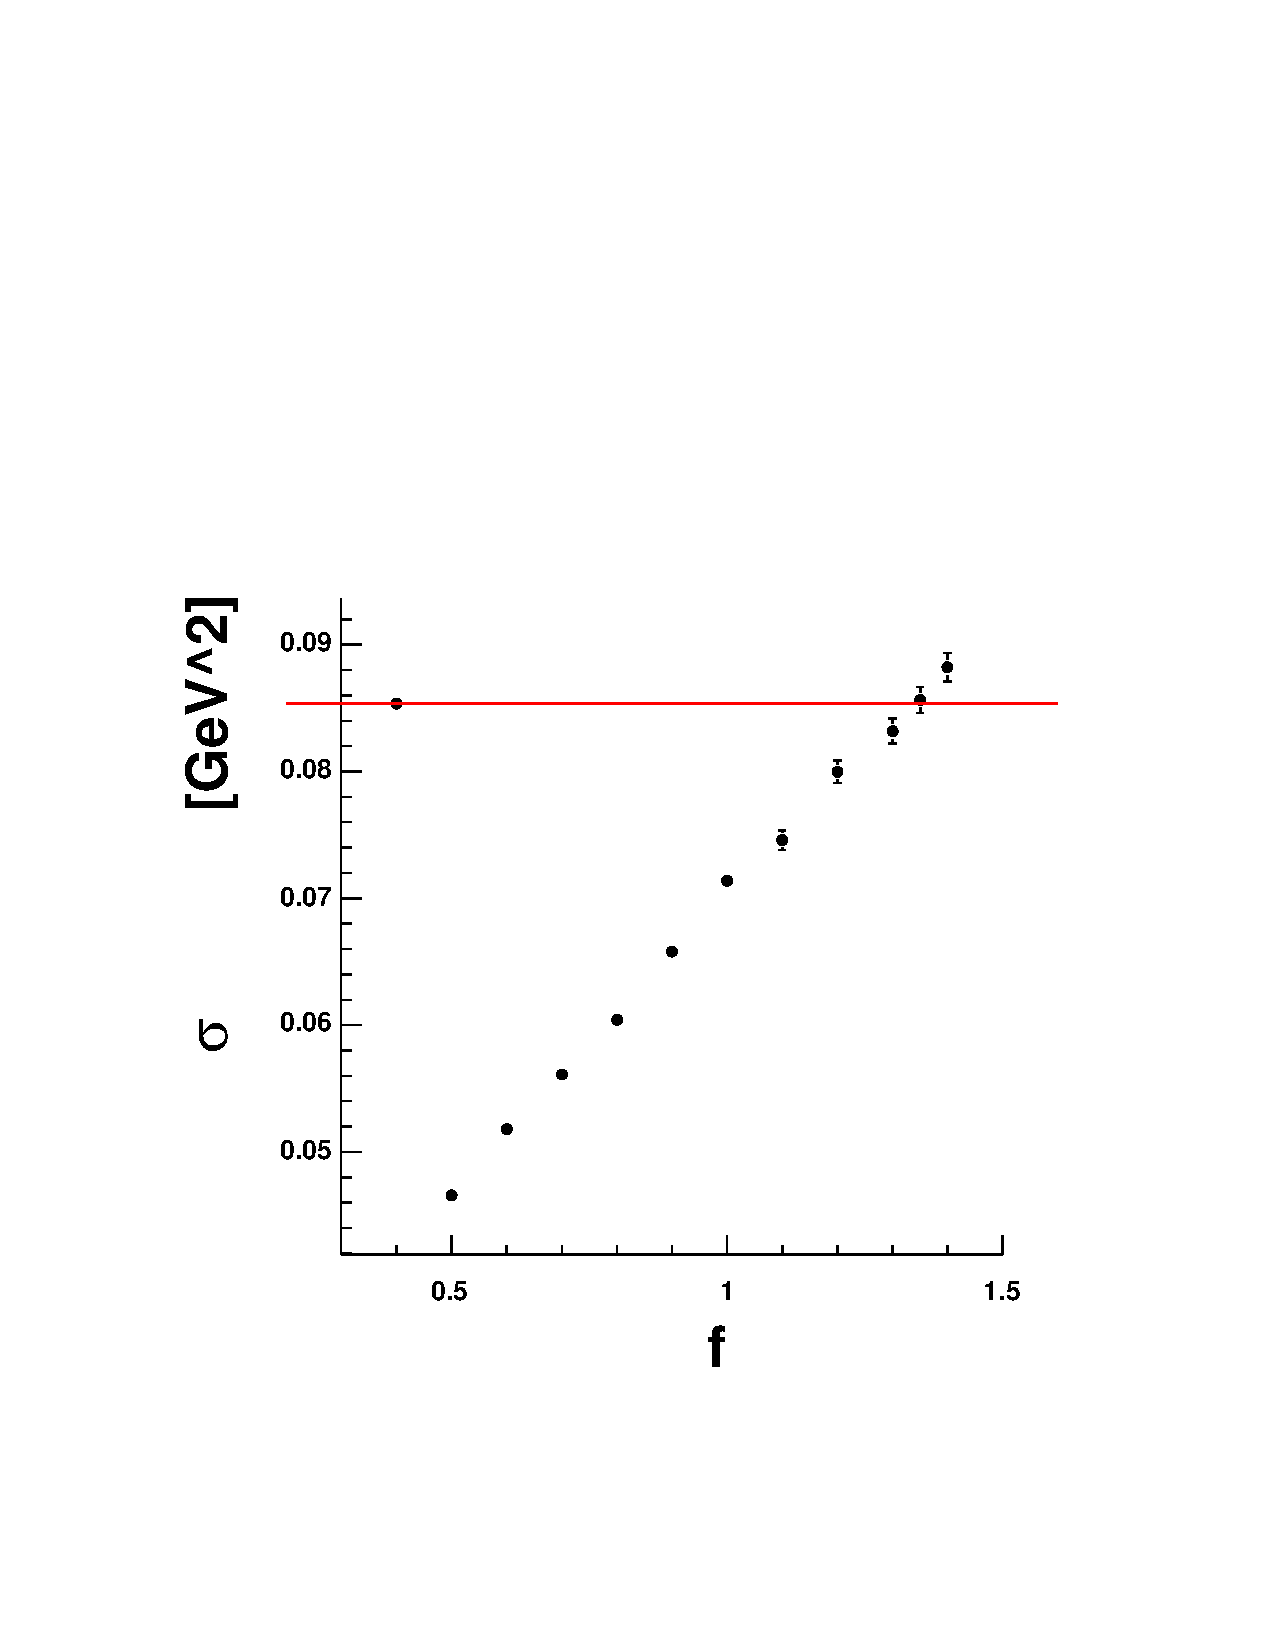
\includegraphics[width = 14cm, bb=0 120 620 540]{acceptance/img/all_com_sc}
 \caption[$\sigma$ as a function of the smearing factor $f$]
         { $\sigma$ as a function of the smearing factor $f$. The first point is the
	            real data resolution (red line). The real resolution is matched at $f=1.35$.}
 \label{fig:tof_fit}
\end{figure}



